\documentclass[tikz,border=2mm]{standalone}
\usepackage{amsmath}
\usetikzlibrary{shapes.geometric, positioning, calc, arrows.meta}

\begin{document}

% 1. Feladat (Házikó)
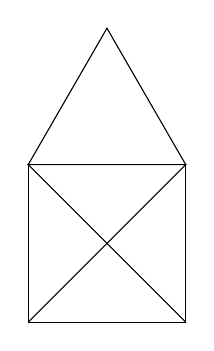
\begin{tikzpicture}[scale=2]
    % Koordináták
    \coordinate (A) at (0,0);  % bal alsó sarok
    \coordinate (B) at (1,0);  % jobb alsó sarok
    \coordinate (C) at (1,1);  % jobb felső sarok
    \coordinate (D) at (0,1);  % bal felső sarok
    \coordinate (T) at ($(D)+(60:1)$); % Tetőpont (D-ből 60 fokra 1 egység)

    % Házikó alap
    \draw (A) -- (B) -- (C) -- (D) -- cycle;

    % Tető rajzolása (két vonal, amelyek találkoznak a tetőcsúcson)
    \draw (D) -- (T) -- (C);

    % Házon belüli két vonal, ami metszi egymást
    \draw (A) -- (C) -- (D) -- (B);

\end{tikzpicture}

\vspace{1cm}

% 2. Feladat (Egységkör)
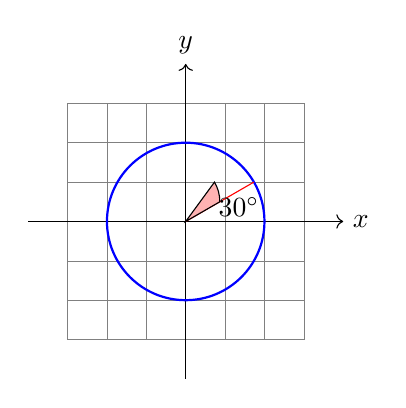
\begin{tikzpicture}
    % Rácsozás
    \draw[step=0.5,gray,very thin] (-1.5,-1.5) grid (1.5,1.5);

    % Tengelyek
    \draw[->] (-2,0) -- (2,0) node[right] {$x$};
    \draw[->] (0,-2) -- (0,2) node[above] {$y$};

    % Egységkör
    \draw[thick,blue] (0,0) circle (1);

    % Sugár 30 foknál
    \draw[red] (0,0) -- (30:1);

    % Szög kijelölése
    \filldraw[fill=red!30] (0,0) -- (30:0.5) arc[start angle=0,end angle=30,radius=0.5] -- cycle;

    % Szög felirat
    \node at (15:0.7) {$30^\circ$};
\end{tikzpicture}

\vspace{1cm}

% 3. Feladat (Kitöltések)
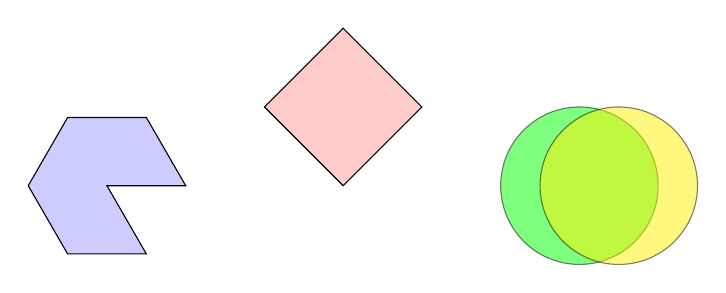
\begin{tikzpicture}
    % Hatszög
    \draw[fill=blue!20] (0,0) \foreach \i in {0,...,5} { -- ({cos(60*\i)},{sin(60*\i)}) } -- cycle;

    % Rombusz
    \draw[fill=red!20] (3,0) -- (4,1) -- (3,2) -- (2,1) -- cycle;

    % Két áttetsző alakzat átfedése
    \filldraw[fill=green,opacity=0.5] (6,0) circle (1);
    \filldraw[fill=yellow,opacity=0.5] (6.5,0) circle (1);
\end{tikzpicture}

\vspace{1cm}

% 4. Feladat (Címkézett egységkör)
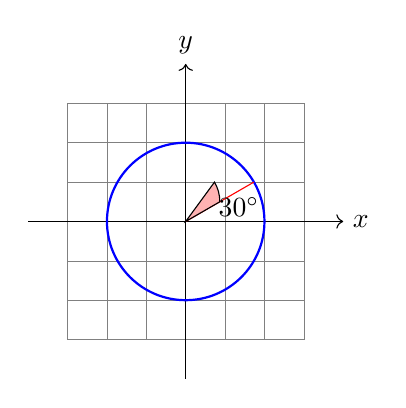
\begin{tikzpicture}
    % Rácsozás
    \draw[step=0.5,gray,very thin] (-1.5,-1.5) grid (1.5,1.5);

    % Tengelyek címkézve
    \draw[->] (-2,0) -- (2,0) node[right] {$x$};
    \draw[->] (0,-2) -- (0,2) node[above] {$y$};

    % Egységkör címkézve
    \draw[thick,blue] (0,0) circle (1);

    % Sugár 30 foknál
    \draw[red] (0,0) -- (30:1);

    % Szög kijelölése és címkézés
    \filldraw[fill=red!30] (0,0) -- (30:0.5) arc[start angle=0,end angle=30,radius=0.5] -- cycle;
    \node at (15:0.7) {$30^\circ$};
\end{tikzpicture}

\vspace{1cm}

% 5. Feladat (Folyamatábra)
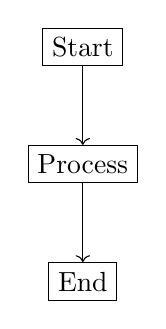
\begin{tikzpicture}
    \node[draw] (start) {Start};
    \node[draw, below=of start] (process) {Process};
    \node[draw, below=of process] (end) {End};

    \draw[->] (start) -- (process);
    \draw[->] (process) -- (end);
\end{tikzpicture}

\vspace{1cm}

% 6. Feladat (Szinusz és koszinusz függvények)
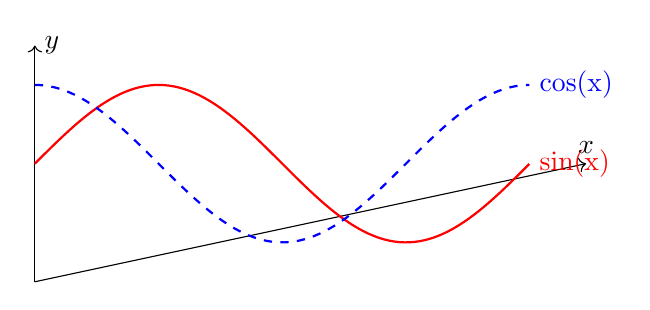
\begin{tikzpicture}
    % Tengelyek
    \draw[->] (0,-1.5) -- (7,0) node[above] {$x$};
    \draw[->] (0,-1.5) -- (0,1.5) node[right] {$y$};

    % Szinusz görbe
    \draw[red,thick] plot[domain=0:6.28,samples=100] (\x,{sin(\x r)}) node[right] {sin(x)};

    % Koszinusz görbe
    \draw[blue,thick,dashed] plot[domain=0:6.28,samples=100] (\x,{cos(\x r)}) node[right] {cos(x)};
\end{tikzpicture}

\end{document}
